\documentclass[12pt, a4paper]{article}
\usepackage[margin=0.75in]{geometry}
\usepackage{graphicx}
\usepackage[utf8]{inputenc}
\usepackage[T1]{fontenc}
\usepackage{amsmath}
\usepackage{algorithm}
\usepackage[noend]{algpseudocode}
\usepackage[style=apa, backend=biber]{biblatex}
\usepackage{color}

\usepackage{caption}
\captionsetup[figure]{font=footnotesize,labelfont=footnotesize}
\usepackage{wrapfig}


\addbibresource{report.bib}
\makeatletter
\def\BState{\State\hskip-\ALG@thistlm}
\makeatother

\parindent=0pt % disables indentation
\parskip=12pt  % adds vertical space between paragraphs

\title{CTA Project}
\author{Fiachra O'Donoghue}

\begin{document}
    
\section{Introduction}

%%%Introduction (10%):  Introduce the concept of sorting and sorting algorithms, discuss the relevance of concepts such as complexity (time and space), performance, in-place sorting, stable sorting, comparator functions, comparison-basedand non-comparison-based sorts, etc.%%%



Formal definition of sorting and the property of being sorted\dots
Sorting: reorganising a list, A,such that if A\textsubscript{i} < A\textsubscript{j} then i < j must be true.enwiki:997404113


If there exists any pair of elements in a collection A, at positions \emph{i} and \emph{j}, such that \emph{i} < \emph{j} but A\textsubscript{i} > A\textsubscript{j} -- with respect to whatever comparator function is relevant -- that pair of elements is known as an inversion. The degree of disorder or "unsortedness" of a collection of elemetns is measured by the number of inversions present.

To be sorted: Each item in the collection is less than or equal to its successor.

Equal-valued elements must be contiguous; i.e. if A\textsubscript{i} = A\textsubscript{j} then there must be no k such that i < j < k and A\textsubscript{i} $\ne$ A\textsubscript{k}

The contents of a collection, A, must be the same before and after searching; i.e. the sorted collection A must be a permuattion fo the pre-sorted collection A.

<, =, $\ne$, and > can be interpreted in terms of mathematical equality or any othey arbtrary but well defined system of ordering. It should be possible to define a \emph{comparator function} which can take two elements, say \emph{a} and \emph{b}, and return a value based on whether \emph{a} < \emph{b}, \emph{a} > \emph{b}, or \emph{a} = \emph{b}.

Sorting algorithms, in general, operate independently of the precise definitions of \emph{less than}, \emph{greater than}, and \emph{equal to} differing instead in how they go about making comparisons between pairs of elements with the goal of a completely sorted collection.

The particular problem's definition of equivalence is encoded in the comparator function and the precise nature of the comparator function is irrelevant to the sorting algorithm which merely requires a black box through which it can pass two values and which returns a codification of the equivalence of those values.

More concretely; the following pseudocode demonstrates a comparator function which for comparing numerical values.

\begin{algorithm}
\caption{A function for comparing numerical values}\label{euclid}
\begin{algorithmic}[1]
\Procedure{Comparator}{a, b}
\If {$a < b$} \Return -1
\EndIf
\If {$a = b$} \Return 0
\EndIf
\If {$a > b$} \Return 1
\EndIf
\EndProcedure
\end{algorithmic}
\end{algorithm}






\subsection{Analysing algorithm complexity}

Worst, Best, and Average cases.
These are classes of inputs, specific to a particular algorithm, for which that algorithm exhibits its least efficient, most efficient, and most usually efficient performances, respectively. In practice, best and worse cases are uncommon, but algorithms are often compared and chosen based on their worst case performances as this defines the lower bound on the algorithm's efficiency.

Generally speaking, the performance of an algorithm vis-$\acute{a}$-vis the number of operations it must perform or the time it takes to complete its task, can vary significantly over all possible input combinations of size \emph{n}. The worst cases are those instances where the algorithm performs the greatest number of operations or takes the longest time, over of all of those input instances. Worst case offers a guarantee that an algorithm will perform no worese - will take no longer - than it does in that case. 


Complexity can be assessed based on use of whatever resources are scarce and need to be optimised for. Most commonly, algorithms are assessed based on time taken, or number of operations, per input size. 
Asymptotic Notation
In algorithm analysis, Big O notation (e.g. O(n$\textsuperscript{2}$)) describes the performance of an algorithm in the worst case scenario. This can be used to classify algorithms by complexity - two algorithms with the same Big O complexity will perfom similarly in their worst cases, and, of two algorithms with different Big O values, the one with the lesser value will perform much more efficiently in its worst case than the other will in its own worst case.

Tightest upper bound should be specified

Omega ($\Omega$) notation represents the complexity of an algorithm in its best case, and Theta ($\Theta$) notation represents its complexity in the average, or most usual case

In describing an algorithm in terms of efficiency, it is necessary to isolate its description from its specific implementation. It is therefore analysed in terms of \emph{n}, the number of elements in, or the size of, its input, and \emph{f(n)} - the runtime, or the number of operations it takes to complete its task, given \emph{n}. All elementary operations are assumed to take the same amount of time.
Some algorithms can have good time complexity but are not practical for certain kinds of input data, e.g. insertion sort performs poorly on lage datasets but extemely well on smaller ones.

Where an implementation requires the use of nested loops, in most cases this will indicate O(n\textsuperscript{2}) complexity.

A priori analysis -- theoretical perspective --- independent of implementation details -- compare order of growth between algorithms -- ***measure of complexity.***

A posteriori analysis -- empirical evaluation of implementation of  algorithm -- ***tied to implementation an platform*** -- performance compared --- *** measure of performance ***

External factors affecting time of execution but not connected to complexity:
Size of intpu, speed of computer, quality of compiler.

To sum up: Performance vs complexity
Performance: how much memory, time, etc is used when algorithm is run --- depends on external factor as well as code 
Complexity: How resource requirements scale as input gets larger

Complexity affects performance but performancedoes not affect complexity

Because algorithms are platform independent, empirical analyses cannot necessarily be generalised to all combinations of platform, etc.... so an independent measure of complexity is necessary to compare algorithm performance. This measure can be assigned to a number of orders of magnitude. 

Complexity families:
    Constant, Logarithmic (log n), Sublinear, linear, n log(n), Polynomial, exponential

To evaluate complexity, most expensive computation should be identified, and the order of that computation will be the order of the complexity of the algorithm.

--- Higher order term will dominate 

\subsection{Sorting algorithm properties}

\subsubsection{Stability}

Stability is the property whereby two equally valued elements in the input collection maintain their positions with respect to one another in the output (sorted) collection. Stability is unlikely to be an important consideration when sorting a collection of simple objects such as numbers but, when there is satellite data, it can become important \autocite{cormen01}.

\subsubsection{Time efficiency}
Time efficiency and space efficiency --- how we compare and rate algorithms



\subsubsection{Memory efficiency}
In-place sorting: Only a fixed amount of memory over the size of n (size of input) required, regardless of size of n. Non-in-place algorithms generally need an amount of memory that increases monotonically with n.

\subsubsection{Suitability for a particular input}

e.g. Size of input, degree of sorting, domain of input (e.g. integers from 1 to 1000), memory requirements, storage location (e.g. external?)

In addition to size of input, specific characteristics of the input can affect the performance of an algorithm. For instance, given two sorting algorithms, one may outperform the other on an input with very few inversions, while the other may be more efficient given an input which is less sorted initially. Similarly, one algorithm may perform particularly well on smaller inputs while performing poorly on larger ones. Insertion sort, for example, examined in more detail below, performs extremely well on input sizes up to ~n=20 but performance falls off as n increases giving it by far the worst overall performance of the five algorithms examined here. The differential efficiency depending on input characteristics can be exploited by algorithm designers to make highly efficient adaptive hybrid algorithms which switch strategy to best tackle the particular nature of the part of the input data on which they are currently working. Timsort, for instance, reduces the number of comparisons made by identifying and merging (using a merge sort) pre-existing runs in its input, and will add to those runs, where they are below a minimum threshold, using insertion sort which is very efficient on small inputs \autocite{enwiki:997404113}. The implementation of introsort used here, described below, uses a recursive partitioning algorithm to divide the sorting task into sublists and switches to heapsort when a maximum recursion depth is reached, as well as to insertion sort when a sublist contains fewer than 20 elements.

It follows from the fact that an algorithm will perform better or worse depending on the nature, as well as on the size of its input, that choice of algorithm does not rest solely on its complexity relative to other competing algorithms. It also depends on the nature of the input in terms of its size, degree of sortedness, and the underlying probability distribution of the specific inputs it is likely to encounter.

\subsection{Comparison Sorts}

Only uses comparison operators to order elements. A comparison based sorting algorithm orders a collection by comparing pairs of elements until the collection is sorted.

No comparison sorting algorithm can perform better than \emph{n log n} in the average or worst cases. Some non-comparison based sorting algorithms can, under certain circumstances, with better worst-case times than \emph{n log n}.

\subsection{Non-comparison Sorts}

\section{Sorting Algorithms}

%%%Introduce  each  of  your  chosen  algorithms in  turn,  discuss their  space  andtime complexity, and explain how each algorithm works using your own bespoke diagrams and different example input instances.  If you diagrams are not original creationsyou will get zero.%%%

\subsection{Insertion sort}


\begin{wrapfigure}{r}{0.3\textwidth}
    \centering
    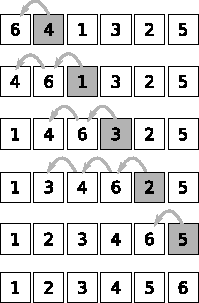
\includegraphics{insertion_sort.pdf}
    \caption{\label{fig:insertion_sort}Insertion sort.}
\end{wrapfigure}

Insertion sort is a comparison sort algorithm which works in linear time in best case ($\Omega$(n)), i.e. an already sorted input, and quadratic time in the average and worst cases ($\theta$(n$\textsuperscript{2}$) and $O(n\textsuperscript{2}$)). The algorithm sorts in-place so space complexity is constant. It is efficient when sorting small or almost sorted inputs, and where there are many duplicate elements \autocite[p. 60]{heineman2016algorithms}.

The algorithm consists of two loops, one nested inside the other. The outer loop iterates from the second element in the input list to the end. If the index of the current outer loop value is \emph{i}, the inner loop compares the value at \emph{i}, known as the \emph{key} with the value to its left (\emph{i - 1}). If the element at \emph{i - 1} is less than, or equal to, the key, no action is necessary as the two elements are sorted with respect to one another. However, if the value at \emph{i - 1} is greater than the key then the value at \emph{i - 2} is compared with the key, and the inner loop continues leftward until either the beginning of the list is reached or a value smaller than the key is found. When this occurs, the key is inserted into the appropriate slot in the list and all of the elements that were compared with it and found to be larger are shifted one position to the right.

Figure \ref{fig:insertion_sort} demonstrates the insertion sort operating on an unsorted list of six digits. Each row represents an iteration of the outer loop. The key in each iteration is represented by the grey box. The red arrow denotes the insertion of the key into its new position, and the grey arrows represent the shifting of all of the intervening, larger, values one position to the right. Note that the elements to the left of the key are always sorted with respect to one another, while the elements to the right of the key have yet to be inserted into this sorted sub-array. Note also that each grey arrow represents one iteration of the inner loop. The inner loop needs to run once only for each inversion of which the current key is a part. This is why the algorithm has a running time of $\Omega$(n) for an already sorted list — because a single run of the outer loop — \emph{n} - 1 iterations — with one comparison per iteration, and without any iterations at all of the inner loop, will confirm that the input is sorted.

The worst case running time is equal to $n \times (n - 1) \times \frac{1}{2} = \frac{n\textsuperscript{2} - n}{2}$ and the average case time is  $n \times (n - 1) \times \frac{1}{4} = \frac{n\textsuperscript{2} - n}{4}$ \autocite{woltmann20:insertion}. Taking only the highest order term into account as this will be the dominant term as \emph{n} grows, this gives us average and worst case performances of $\theta$(n$\textsuperscript{2}$ and $O(n\textsuperscript{2}$). Finally, the algorithm is stable, as if the algorithm encounters a value equal to the key to the key's left, it will simply move back to the outer loop and onto the next element, leaving the two equal elements where they are.

\subsection{Quicksort}

\begin{wrapfigure}{R}{0.4\textwidth}
    \centering
    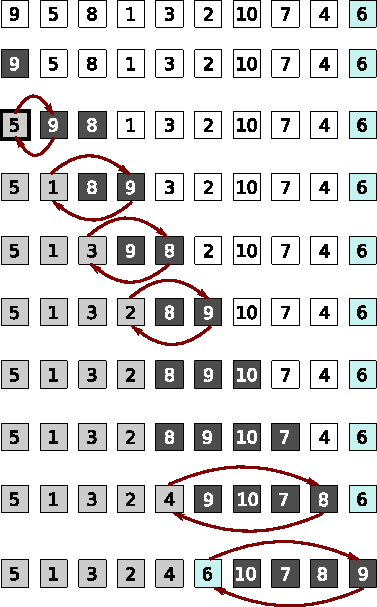
\includegraphics{quicksort.pdf}
    \caption{\label{fig:quicksort_1}Quicksort partitioning.}
\end{wrapfigure}

Quicksort is a comparison sorting algorithm which recursively partitions its input data based on whether each element is higher or lower than a sometimes arbitrarily chosen \emph{pivot} value. The algorithm runs in $n\log n$ time in the best and average cases, and $n^{2}$ time in the worst case.

Figure \ref{fig:quicksort_1} illustrates the partitioning mechanism of the algorithm. First a pivot is chosen. Much can be said on the subject of pivot selection, and the matter is discussed below, but for the purposes of this demonstration, the pivot is taken to be the last element of the input array. The pivot value is highlighted in blue. As the algorithm progresses, each value in the array is compared to the pivot value. If the current value is greater than the pivot value it is assigned to the right-hand sub-array — represented by the dark boxes in figure \ref{fig:quicksort_1}. If the current value is less than the pivot value then it is swapped with the first value of the right-hand sub-array. Finally, when the pivot value, which is located in the last array position, is reached, it is swapped with the first value of the right-hand sub-array. This places it between a sub-array containing only values smaller than it, and a sub-array containing only values that are equal to or exceed it. It also places it in the position it will occupy in the fully sorted array. The partitioning portion of the quicksort algorithm will then return the location of the pivot value so that two recursive calls to quicksort can partition one of the two sub-arrays each.

\begin{wrapfigure}{R}{0.4\textwidth}
    \centering
    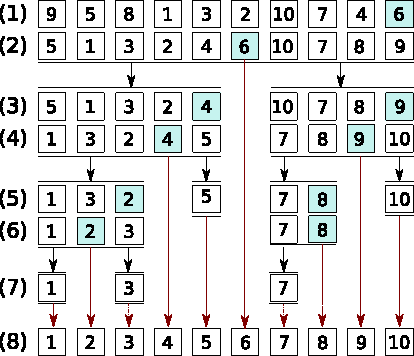
\includegraphics{quicksort_2.pdf}
    \caption{\label{fig:quicksort_2}Quicksort sorting.}
\end{wrapfigure}

Figure \ref{fig:quicksort_2} illustrates the overall operation of quicksort. The first two rows shoe the original array to be sorted and the result of the call to the partition algorithm shown in figure \ref{fig:quicksort_1}. After partitioning, the original pivot value, 6, is in its final sorted position. The two sub-arrays on either side of 6, one containing only values less than and one containing only values greater than, 6. The last value in each array is again chosen as the pivot (row 3) and both subarrays are again partitioned (row 4). The two pivot values, 4 and 9, for the sub-arrays partitioned in row 4 are now in their final sorted positions. Of the four sub-arrays produce by the partitioning in row 4, two contain just a single value, meaning that they are now in their final sorted positions; numbers 5 and 10 are now sorted. The remaining two sub-arrays are partitioned, producing two more sorted pivot values, 2 and 8 (row 6), and three single-element arrays (1, 3, and 7), completing the array sort. 

The array has been sorted in-place, without any overhead, giving a space complexity of \emph{n}. As for time complexity, it has already been mentioned that quicksort finishes in $n\log n$ time for best and average cases. \textcite[119]{bentley:pearls} makes the point that as comparison algorithms, such as quicksort, are provably limited to $O(n\log n)$, quicksort's performance is ``close to optimal.''  He goes on to say, however that the algorithm's performance degrades to $O(n^{2})$ given some common inputs such as an array with long runs of identical elements.

Poorly chosen pivot values can cause poor performance. Performance is likely to be best — all else being equal — when the pivot, for the most part, is located near the middle of the data, so that the two partitioned sub-arrays are of roughly size. This being the case, suggests \textcite[851]{Sedgewick-1978}, the median may be an optimal value for the pivot, and he goes on to outline a method for sampling three values — the first, the last, and the middle, from each array or sub-array to be partitioned, and setting the pivot value to the median of those three. Other frequently used values are the first value in the array, the last value, or a random value \autocite*[73]{heineman2016algorithms}.

One final interesting optimisation, attributed without citation by \textcite[121]{bentley:pearls} to Sedgewick, is the use of insertion sort to sort small sub-arrays for which quicksort would be inefficient. The suggested implementation would entail halting partitioning when array length fell below a certain threshold, and using insertion sort to complete sorting of the almost-sorted final array. This solution starts to resemble introsort \autocite{musser1997}, which is discussed below in section \ref{sec:introsort}.


\subsection{Heapsort}

Heapsort is a sorting algorithm that sorts data by first rearranging it so that it forms a \emph{max-heap}, taking the top value, then recursively rearranging the remaining elements into a max-heap and taking the top value until the heap is exhausted and the array is sorted. The algorithm runs in $O(n\log n)$ time in the best, average, \emph{and} worst cases. It sorts in-place so its space complexity is $O(1)$ \autocite[129]{cormen01}.

A heap is a binary tree which is completely filled, with the possible exception of the lowest level, which, to the extent it  \emph{is} filled, is populated from left to right, with the rightmost nodes filled last. A max-heap is a heap in which the value of every node, with the exception of the root node, is less than or equal to that of its parent \autocite[127-129]{cormen01}. A max-heap can be stored as 1-based array with the root node at index, \emph{i} = 1 and such that given the index \emph{i} of any node, the parent of that node will be at \emph{i}/2, and its left and right children will be at 2\emph{i} and 2\emph{i} + 1, respectively \autocites[128]{cormen01}[148]{bentley:pearls}. In the implementation used here, however, the root node is stored at \emph{i} = 0, putting a node's parent at (\emph{i}-1)/2, and its left and right children at 2\emph{i} + 1 and 2\emph{i} + 2, respectively. An example of a max-heap can be seen in figure \ref{fig:heap}.


\begin{wrapfigure}{r}{0.4\textwidth}
    \centering
    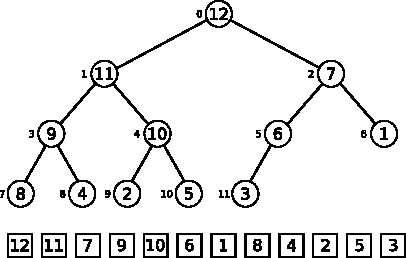
\includegraphics{heap.pdf}
    \caption{\label{fig:heap}A max heap generated from an array holding the numbers 1 to 12. The small number to the left of each node is the index of that node's value in the array below.}
\end{wrapfigure}

Any array can be seen as a heap. Note the array indices attached to the heap nodes in figure \ref{fig:heap}; the nodes are simply filled from top to bottom, and left to right. Rearrangement of the heap, (i.e. rearrangement of the underlying array) so that it complies with the requirement that each parent node be greater than or equal to both of its child nodes, will produce a max-heap. The heapsort algorithm sorts an array, A, by repeatedly forming a max heap and removing the top node — which, by definition, is the greatest value in the array, and which will be located at position A[0]. The removed maximum value is swapped with the value at the end of the array. From this point the array is split into a heap sub-array and a sorted sub array. At each iteration of the algorithm, the greatest remaining value in the heap sub-array is identified by rearrangement of that sub-array into a max-heap, and is swapped with the last value in the heap sub-array. Thus, the sorted sub-array grows larger and the heap sub-array grows smaller, until the array is fully sorted. Figure \ref{fig:heapsort} illustrates the process.

\begin{figure}[H]
    \centering
    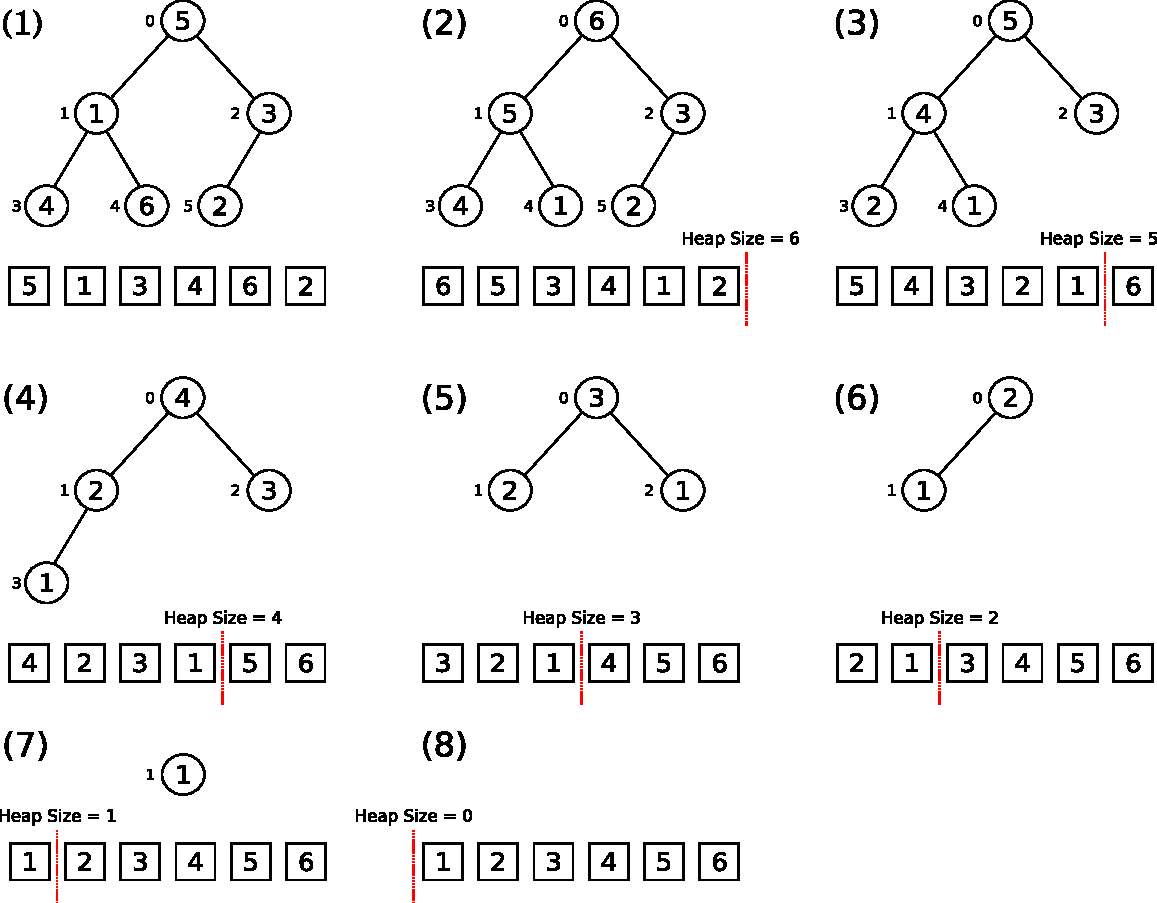
\includegraphics[height=10cm]{heap_sort2.pdf}
    \caption{\label{fig:heapsort}The process of sorting a 6 element array using heapsort: (1) the original array viewed as an array and as a heap; (2) the array rearranged as a max-heap; (3) the in the max-heap is swapped with the last value in the array. A new max heap is formed; (4-6) max heaps are formed, top value is swapped into last position of heap sub-array, heap-size is decremented; (7) max-heap of 1 node is   ``swapped'' into the sorted subarray; (8) the sorted array.}
\end{figure}





\subsection{Counting sort}

\begin{wrapfigure}{r}{0.4\textwidth}
    \centering
    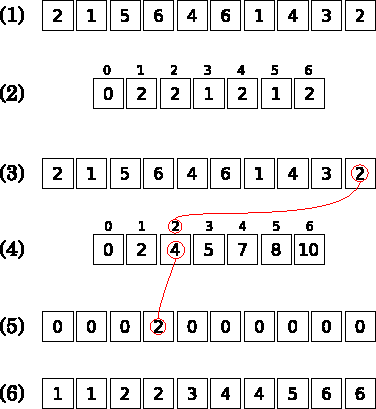
\includegraphics{counting.pdf}
    \caption{\label{fig:counting}The process of a counting sort algorithm: (1) The array to be sorted; (2) The counter array — the value at index \emph{i} is incremented when the value \emph{i} is encountered in the input array; (3) the input array is iterated through in reverse; (4) the count array now holds a cumulative sum of counts; (5) the output array is populated using the cumulative sum of counts — effectively showing positions of last occurrences of values; (6) cumulative counts are decremented as they are used, and the sorted output array is populated.}
\end{wrapfigure}

Counting sort is the first non-comparison sort reviewed here. The algorithm sorts data by counting the number of occurrences of each unique value in the input and then calculating the index in the sorted output of the last incidence of each value. With this information it is able to populate a sorted output list. Counting sort runs in $O(n)$ time when the range of possible values, \emph{k} is $O(n)$ \autocite[168]{cormen01}

Counting sort must know the range of values, \emph{k} in its input data. When it is passed an array for sorting, the algorithm creates two further arrays: a count array, of length \emph{k} and an output array equal in length to the input array. The algorithm begins by iterating through the input. On each value it encounters


\subsection{Introsort}\label{sec:introsort}

Added insertion sort when partition size <= 20 


\section{Implementation \& Benchmarking}

Re insertion sort slower on value based as opposed to refernce based-- python interns first 255 unsigned? --- so ref based

Benchmarking: empirical method for comparing algorithm performance a postiori. Can be used to vaildate a priori / theoretical hypotheses

@max Use the min() rather than the average of the timings. That is a recommendation from me, from Tim Peters, and from Guido van Rossum. The fastest time represents the best an algorithm can perform when the caches are loaded and the system isn't busy with other tasks. All the timings are noisy -- the fastest time is the least noisy. It is easy to show that the fastest timings are the most reproducible and therefore the most useful when timing two different implementations.



\begin{table}[h]
    \resizebox{\textwidth}{!}{%
    \begin{tabular}{rrrrrrrrrrrrrr}
\hline
             \textbf{\emph{n}=} &   \textbf{100} &   \textbf{250} &   \textbf{500} &   \textbf{750} &   \textbf{1000} &   \textbf{1250} &   \textbf{2500} &   \textbf{3750} &   \textbf{5000} &   \textbf{6250} &   \textbf{7500} &   \textbf{8750} &   \textbf{10000} \\
\hline
 \textbf{Insertion sort} &          0.579 &          3.639 &         14.431 &         34.790 &          58.874 &          93.975 &         367.431 &         831.598 &        1460.917 &        2496.221 &        3437.074 &        4970.057 &         8248.562 \\
      \textbf{Quicksort} &          0.404 &          1.015 &          2.283 &          3.815 &           5.511 &          10.473 &          28.061 &          42.266 &         106.330 &         161.203 &         118.821 &         140.753 &          170.012 \\
       \textbf{Heapsort} &          1.098 &          3.367 &          7.923 &         13.440 &          14.017 &          21.729 &          47.937 &          76.649 &         110.026 &         135.903 &         165.639 &         107.672 &          234.757 \\
  \textbf{Counting sort} &          0.170 &          0.345 &          0.733 &          1.120 &           1.460 &           1.782 &           3.371 &           4.957 &           5.874 &           7.693 &           9.523 &          11.409 &           13.184 \\
      \textbf{Introsort} &          0.544 &          1.268 &          1.974 &          2.274 &           3.355 &           4.059 &          19.723 &          52.953 &          78.816 &         101.914 &         117.982 &          75.824 &           78.587 \\
\hline
\end{tabular}
    }
\caption{Times in milliseconds to sort arrays of size \emph{n} for each of the algorithms}
\end{table}

\begin{figure}
    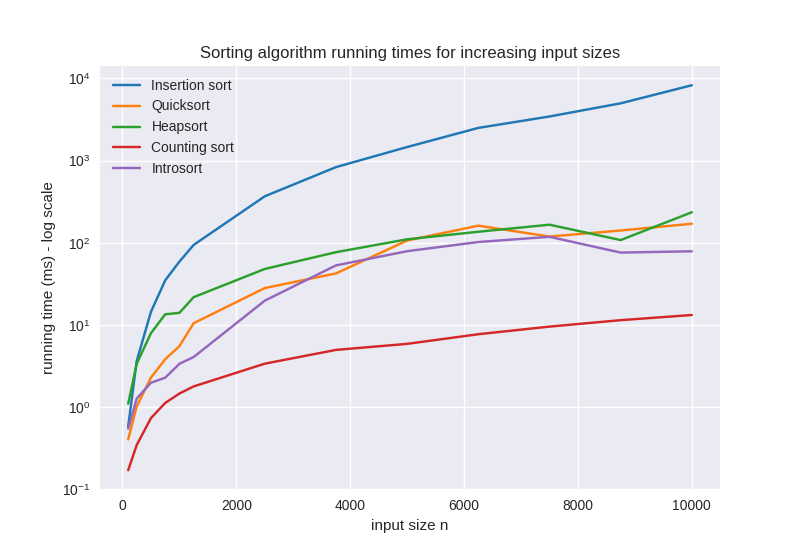
\includegraphics[width=\linewidth]{bm_output/plot_0_log_20210510-153504.png}
    \caption{Relative performance of algorithms using a log y-scale.}
    \label{fig:log-perf}
  \end{figure}


https://www.oreilly.com/library/view/python-cookbook/0596001673/ch17.html 
-- Tim Peters on timing \textcite{peters2002}
"The slowest result is often computed on the first try, because your machine’s caches take extra time to adjust to the new task."




\printbibliography
\end{document}